\chapter{O contexto da relação cinema e pintura --- o movimento em direção ao espaço}%
\label{cap1-contexto-relacao-cinema-pintura}
\pagestyle{headings}

\section{Perspectiva histórica}%
\label{sec-perspectiva-historica}

Antes de prosseguirmos com o esclarecimento dos conceitos de movimento
e espaço, do ponto de vista teórico, é necessário definir de que cinema
e de que pintura estamos tratando. Iniciamos, assim, uma breve
contextualização. O resgate do momento histórico do encontro dos
primeiros filmes com a representação pictórica tradicional, do início
do século XIX, nos forneceu o contexto para dar início a esta
investigação, que tem como objeto o filme clássico narrativo e a
pintura em tela. Muitas das primeiras teorias do cinema têm foco na
\emph{Imagem em Movimento}, e são escritas pelos próprios cineastas. As
comparações com a pintura e com teorias da imagem já são evidentes
naquele momento e evoluem para as discussões sobre a impressão de
realidade proporcionada pelo filme. 
Na clássica antologia de \textcite{xavier1983experiencia}, \emph{A
	Experiência do Cinema}, é proposto o recorte de uma teoria do cinema,
já bastante complexa na época. Este recorte se inicia com o estudo do
psicólogo alemão Hugo Münsterberg (1863--1916) sobre como funciona a
narração cinematográfica e as operações mentais do espectador em
relação à atenção, a memória e imaginação e as emoções.\footcite[Para
	saber mais sobre Münsterberg e Rudolf Arnhein, consulte][]
  {pedro2013percepcao} Inclui artigos de outros autores com a
marca do \emph{retorno a Freud}, característico de parcela considerável
dos teóricos das artes a partir dos anos 60. Mas
\textcite{xavier1983experiencia} não se limita a estes dois aspectos,
em sua seleção de textos que se esforçam em
\textcquote[10]{xavier1983experiencia}[.]{demonstrar que a estrutura do
	filme --- entendida como configuração objetiva de imagem e som
	organizados de um certo modo --- tem afinidades diretas com estruturas
	próprias ao campo da subjetividade}. Aborda o problema da ficção, tal
qual se consolidou a partir do cinema narrativo clássico, argumentando
que o produto da indústria pouco mudou em seus princípios, no período
entre 1916 e 1980. Eis, portanto, um elemento fundamental de referência
aqui considerado: a existência de um cinema dominante, rigidamente
codificado, e sua retórica de base --- a
\textcquote{xavier1983experiencia}[.]{impressão de realidade}.

A avalanche de imagens e meios de reprodução ao alcance da palma de
nossa mão, nos dias de hoje, nos fez refletir sobre um outro momento
histórico semelhante, que se inicia com a invenção do cinema. A
construção da pintura e das imagens já tinham seus tratados, que
evoluíram e acompanharam a própria história da cultura ocidental. No
entanto, no final do século XIX, nos anos da plenitude das descobertas
tecnológicas a serviço da revolução industrial, o cinema funda uma nova
forma de se pensar a imagem (Berger, 1972). O período crítico da
pandemia (2019--2021), quando milhares de imagens invadem a casa e a
vida do espectador, através de avanços tecnológicos, fortemente
pautadas pela propaganda, nos fornece o link presente na relação do
cinema com as vanguardas históricas da pintura no pré e pós I Guerra
Mundial. Realizar esta associação é inevitável, e iniciamos o recorte
temporal nos anos vinte do século XX, diante do movimento
impressionista do cinema de Abel Gance, Jean Epstein, Louis Delluc e
Marcel l'Herbier, que tinha em comum uma reação ao caráter agressivo do
Expressionismo, conforme aponta Isabel Nogueira (2011). A poética
subjetiva e onírica destes filmes retratava temáticas da vida
quotidiana com o mesmo cuidado em relação a questões da luz e
enquadramento, de pintores Impressionistas do século anterior. A
estética dos filmes remontava ao efeito momentâneo da luz \emph{en
	plein air}, a poética e a magia da cor de pintores como Manet, Monet e
os cerca de 30 artistas da \emph{Société Anonyme des Artistes Peintres,
	Sculpteurs, Graveurs}, oficialmente inaugurado no estúdio do fotógrafo
Nadar, em Paris, 1874. \parencite{nogueira2011cinema}.

Na Alemanha, no ano de 1905, foi criado o grupo \emph{Die Brücke} (A
Ponte), pelos artistas Ernst Kirchner (1880--1938), Erich Heckel
(1993--1970) e Karl Schmidt-Rottluff (1884--1976),
\enquote{inaugurando} o Expressionismo na pintura. O movimento surge
como uma reação ao positivismo dos Impressionistas~e seu esmero técnico
com relação às percepções de luzes e cores. A valorização da expressão
emocional e~subjetiva~do ser humano tem seu maior representante na
composição de \emph{O Grito}, que teve diversas versões entre 1893 e
1910, com diferentes técnicas e materiais. Outro grupo Expressionista
que se formou neste período foi \emph{Der Blaue Reiter} (O cavaleiro
azul), em 1911, formado por Franz Marc (1880--1916) e Wassily Kandinsky
(1966--1944).

A história, o cinema e a pintura caminham juntas, e em 20 de fevereiro
de 1909 Filippo Tommaso Marinetti (1876--1944) lança o \emph{Manifesto
	Futurista}. Os conceitos futuristas vêm do domínio da física, como
potência, velocidade e dinamismo. Defensor da rebelião, do amor ao
perigo, da coragem, da audácia, o escritor e poeta cultuava a violência
e a guerra, devido ao seu patriotismo extremista. Como o próprio nome
indica, o grupo rejeitava o passado, acreditando no progresso da
civilização, e na força da sociedade industrializada. Em 1910, o
segundo manifesto resulta do encontro do poeta com os pintores Carlo
Carrà, Luigi Russolo, Gino Severini, Umberto Boccioni e Giacomo Balla.
Neste, propõem igualmente lutar contra a tradição artística, e
inclusivamente contra o próprio Cubismo, fazendo a apologia da máquina,
da velocidade, da luz e da sensação dinâmica. O Futurismo é a
concretização da pesquisa no espaço bidimensional, para expressar o
movimento real, registrando a velocidade descrita pelas figuras em
movimento no espaço, como por exemplo a de um automóvel \parencite{imbriosi2022}.

\begin{displaycquote}[144]{nogueira2011cinema}[.]
	\textelp{} em 1916, aparecia o \emph{Manifesto del cinema futurista},
	assinado por Marinetti, Bruno Corra, Emilio Settimelli, Arnaldo Ginna,
	Giacomo Balla e Remo Chiti. A imagem devia conter todos os ruídos e
	movimentos do mundo, agora fundidos num universo gráfico. A juventude do
	cinema seria, compreensivelmente, o meio privilegiado para satisfazer os
	desejos futuristas. Porém o movimento perdeu continuidade com a I Guerra
	Mundial e os escassos filmes futuristas desapareceram em quase sua
	totalidade
\end{displaycquote}

No Brasil, os ideais da Semana de Arte Moderna que inauguraram o
movimento modernista no país, sofreram influência do Futurismo. Isso
porque a rejeição ao passado, bem como o culto do futuro, servira de
base para as ideias modernistas. A partir de 1919, quando se filiou ao
Partido Nacional Fascista, Marinetti passou a usar o dinamismo da
máquina em movimento, alimentada pela eletricidade que iluminava as
grandes cidades e a indústria, para impulsionar a propaganda fascista.
Inspirado pela revolução russa de 1917, outro nome que podemos associar
à pintura futurista é o de Dziga Vertov (1896--1954). O jovem que
iniciou um curso no Instituto Psiconeurológico de Vladimir Bkhterev, em
Petrogrado, se tornou um dos maiores experimentadores e inovadores da
história do cinema. \emph{Kino-Pravda} (Cine-Verdade) foi uma série de
23 documentários realizados e lançados entre maio de 1922 e março de
1925. Vertov acreditava que o filme ficcional era elitista e antipático
ao regime comunista, porque criava uma realidade falsa. Esta série é
considerada um laboratório para o desenvolvimento de um vocabulário
cinematográfico, com experimentações técnicas, que visavam livrar o
cinema de \emph{elementos burgueses}. Em 1929 realizou o filme \emph{Um
	Homem com uma Câmera}\footnote{Fonte:
	\url{https://www.youtube.com/watch?v=cGYZ5847FiI\&t=5s\&ab\_channel=AllsovietmoviesonRVISION}}
vinculado à arte construtivista do início do século XX, que acolheu o
pensamento do mundo moderno e industrializado, para servir ao bem maior
e coletivo, implantando as novas narrativas visuais. Embora estivesse
inserido na escola soviética de montagem, ao lado de Pudovkin
(1893--1953) e Kuleshov (1899--1970), Vertov defende os filmes de
não-ficção e, em sua crença, a câmera\footnote{Fonte: Manifesto de
	Dziga Vertov (1923) 2:04--3:36
	\url{https://www.youtube.com/watch?v=dijaKEzXzD8\&ab\_channel=PaulaPinheiroMundim}}
é uma peça de tecnologia que serve para interpretar o mundo ao redor,
um super-olho que enxerga e revela além da percepção humana
\parencite{rosebud2020dziga}. Finalizamos este recorte da história, com a
evidência do impacto do cinema, desde o seu estabelecimento enquanto
linguagem, nas artes plásticas.
\textcquote[143]{sabino2000pintura}[.]{Os futuristas revelaram desde
	logo, nas suas pinturas, a absorção das novas imagens em movimento,
	numa pintura algo ciumenta da conquista do cinema (Balla \emph{versus}
	Vertov). Mas tal qual na fotografia, o contrário foi igualmente
	verdade}.

Um último movimento artístico que gostaria de relacionar ao cinema, o
\emph{Dadaísmo}, nasceu durante a primeira Guerra, em 1916, no
\emph{Cabaret Voltaire}, com o manifesto do escritor alemão Hugo Ball
(1886--1927), que com 24 anos estudou na \emph{Max Reinhardt School of
	Dramatic Art}. Curiosamente, o teatro de Max Reinhardt é associado ao
cinema alemão, já em 1913. Segundo \textcite[44]{eisner1985tela}, a
partir de 1907 e até 1919, Max Reinhardt foi um tipo de Kaiser do
teatro em Berlin. Entretanto, ela esclarece que Max Reinhardt,
profundamente \enquote{impressionista}, dispensava as experiências de
choque de luzes e sombras dos expressionistas, que visavam concentrar a
iluminação súbita em um personagem ou objeto. Para Reinhardt, sua
sedutora iluminação \textcquote[46]{eisner1985tela}[.]{tinha o único
	fim de suprimir o verismo e o naturalismo detalhista, caros à geração
	anterior}. \footnote{\textcquote[nota de
		rodapé][46]{eisner1985tela}[.]{Reinhardt, ao se consagrar, antes de
		1914, a mil nuanças e impressões caleidoscópicas, recorria à imaginação~dos
    espectadores. Seu teatro se tornava um amplo espaço onde
		turbilhonava o movimento e uma evolução incessante metamorfoseava a
		vida. Cortinas e panos de paredes dissimulavam parcialmente a curva
		suave de um \emph{Rundhorizont,} de um horizonte cuja superfície
		côncava era inundada ora pelo luar, ora pelos raios de um sol
		resplandecente, para logo mergulhar de novo numa escuridão onde víamos
		oscilar a rede das estrelas, enquanto o jogo de um tipo de lanterna
		mágica a cobria de nuvens movediças}.}

\begin{displaycquote}[44]{eisner1985tela}[.]
	Era natural que o cinema, ao se tornar uma arte, aproveitasse as
	descobertas de Max Reinhardt, que utilizasse o claro-escuro e os mantos
	de luz que se derramavam de uma janela alta num interior escuro, assim
	como eram vistos todas as noites no \emph{Deutsches Theatre}
\end{displaycquote}

Neste contexto teatral, identificamos o possível lançamento da
caracterização do cinema como a arte do espaço, sobre um de seus
pilares que é a construção visual plástica do cenário no espaço
diegético do filme. Em termos gerais, \emph{o} Dadaísmo foi um
movimento de oposição radical, contra a lógica, os valores estéticos
tradicionais e da sua época. Considerado anárquico e provocador, sua
irreverência transparece em duas técnicas artísticas a ele associadas:
a colagem e o \emph{ready-made}. O Dadaísmo chega aos nossos~dias como
um exemplo, não só de contestação de ideias, mas também sobre como
técnicas e processos artísticos são trazidos para os tempos atuais. O
movimento \emph{Dadá} oferecia nexos entre o colecionismo de objetos e
imagens na pintura que investigávamos no ateliê, com alguns aspectos da
montagem no cinema. A poética de acúmulo de imagens que se interligam
por um pensamento em constelação se torna presente em nossos dias, onde
uma complicada rede de referências imagéticas se apresenta por meio da
internet. Olhar para autores contemporâneos como David Salle, Mama
Andersson, William Kentridge, e Adrian Ghenie\footnote{Sobre Adrian
	Ghenie https://www.galeriejudin.com/artist/adrian-ghenie/} nos faz
pensar sobre o conceito de
presentificaçāo\footfullcite{Gumbrecht2010producao} da cultura visual e
memória pessoal do artista.

\begin{figure}
	\caption{\artname{Adrian Ghenie}{Dada is dead}{2009}}

	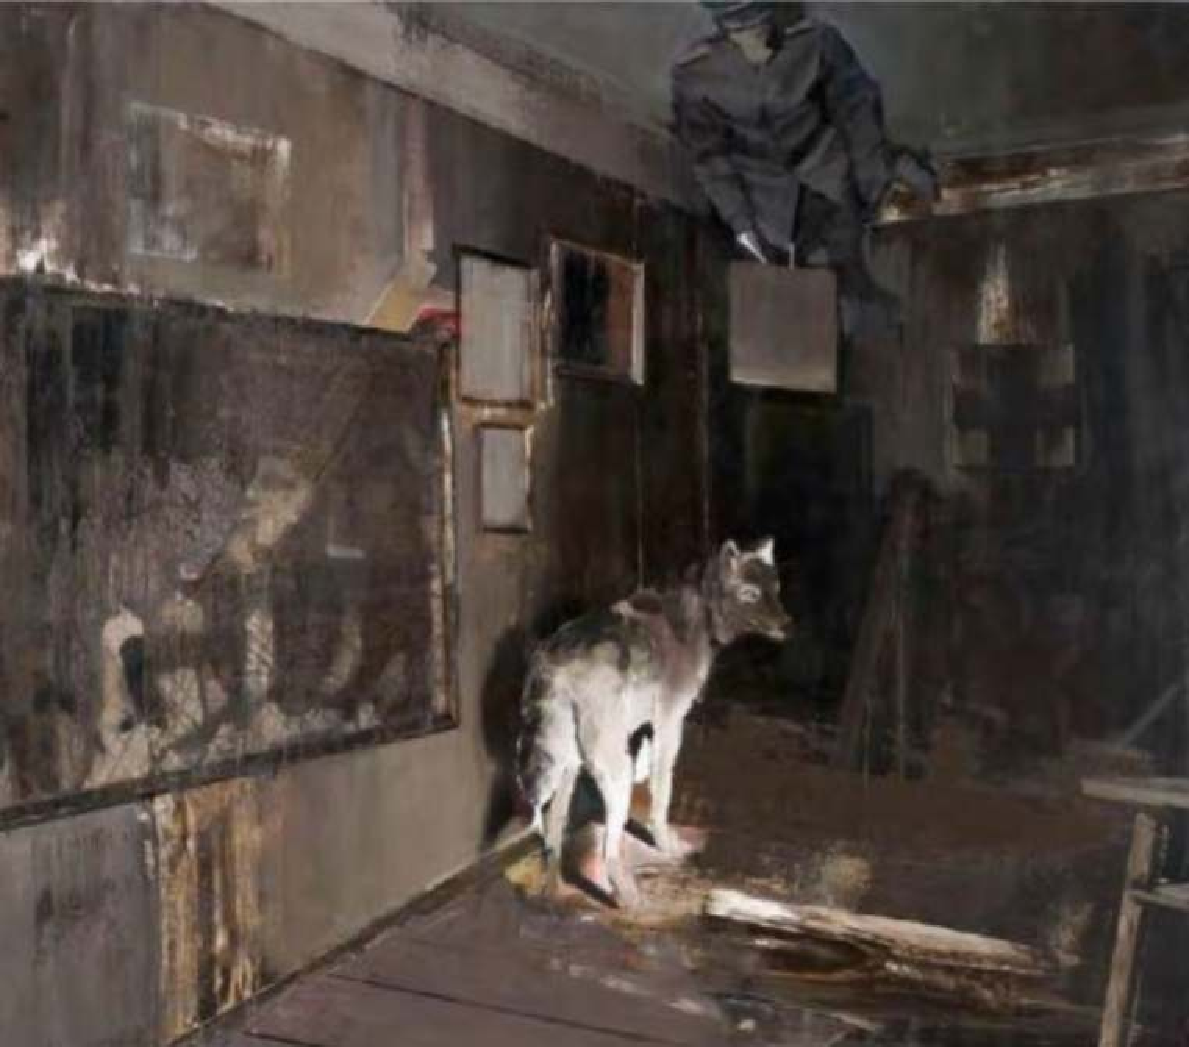
\includegraphics[width=3.98229in,height=3.50617in]{figuras/ghenie-dada-is-dead-2009.pdf.compressed.pdf}
	\figurenote{\oil. \artsize{220 x 200}. Fonte: Adrian Ghenie, 2009 ISBN 978--3--7757--2463--0}
\end{figure}

Não pretendemos nos alongar sobre estes conceitos, mas queremos realçar
a pintura de Adrian Ghenie que faz uma citação histórica ao
\emph{Cabaret Voltaire} na pintura \emph{Dada is dead, 2009}. Detentor
de uma técnica tradicional extremamente avançada, é um dos pintores
contemporâneos mais bem sucedidos. Ghenie (1977) cresceu durante a
ditadura Romena e é representante de uma das primeiras gerações criadas
pela Internet. Esta pintura reflete sua crença de que as vanguardas
então canonizadas estabeleceram uma
\textcquote{judin2022adrian}{atitude extremista na arte, um ódio
	ideológico à pintura. Para mim, o século XX foi um século de humilhação
	--- através da minha pintura, ainda estou tentando entender isso.}

Os assuntos das referências para o artista e a colagem serão retomados
no \cref{cap3-narrativa-visual}, quando abordamos a obra das pintoras
Lucia Laguna e Cristina Canale.

\section{Perspectiva teórica}%
\label{perspectiva-teuxf3rica}

Com a ideia inaugural do cinema como movimento e representação do real,
muitos cineastas e filósofos como Eisenstein, Gilles Deleuze, Rudolf
Arnheim passam a teorizar a imagem sob esta nova perspectiva.
Eisenstein trata o cinema sob o ponto de vista da montagem.
\textcite{deleuze2004imagem}, explora o texto \emph{Matéria e Memória},
escrito em 1896 por Bergson, onde a tônica era a imagem-movimento e a
imagem-tempo, relacionando suas ideias à imagem cinematográfica.
Deleuze avança, ao tratar de questões do espaço como quadro e plano,
enquadramento e decupagem, afirmando sua crença de que o ponto nodal do
cinema é a montagem, que traz em si a ideia do movimento. Segundo
\textcite[49--50]{gil2005atmosfera}, \enquote{Rudolf Arnheim vai se
	insurgir contra os que afirmavam que o cinema era a reprodução da
	realidade\ldots O cinema tem a sua própria representação da
	tridimensionalidade e da profundidade de campo, que nem sempre
	corresponde à percepção visual.}

Nas reflexões sobre como as imagens trabalham para contar histórias, ou
ainda como as histórias conseguem ter seu lugar nas imagens,
\textcite{aumont2004olho} afirma que a pintura sempre pode imitar o
movimento, mas não o tempo, e que este seria um ponto em que a pintura
e o cinema estariam irremediavelmente separados. Por outro lado, Aumont
lembrará a postulação de Rhomer de considerar o cinema como uma arte do
espaço, na sua busca por encontrar um ponto de contato entre o cinema e
a pintura

\begin{displaycquote}[141]{aumont2004olho}[.]
	Eu reclamava para a pintura o direito de ser tratada como uma arte do
	tempo. Trata-se simplesmente, agora, de considerar o cinema como uma
	arte do espaço. A postulação não é nova, nós a encontramos em Eisenstein
	--- onde encontramos tudo ---, mais perto de nós, em Francastel e sobretudo
	em Rohmer\footnote{\emph{Éric Rohmer} (\emph{Maurice Schérer}) escreveu
		no artigo \enquote{\emph{Le cinema, art de l'espace}} (1948) \enquote{O espaço, ao
			contrário (do tempo) parece ser a forma geral de sensibilidade que lhe
			é (ao cinema) verdadeiramente essencial, na medida em que o cinema é
			uma arte da visão.}}, que fez dela, em 1948, um artigo
	propositadamente provocador e paradoxal \textelp{}. Pois encontramos na
	utilização narrativa do espaço por ambos \textelp{} a presença de um mesmo
	implícito: a cena
\end{displaycquote}

Anos depois, em sua tese de doutorado, defendida em 1972, \emph{A
	organização do espaço no Fausto de Murnau}, ele define três tipos de
espaço no cinema.

\begin{quadro}[h]
	\caption{A organização do espaço no cinema por Eric Rohmer}

	\begin{tabular}{lm{.7\linewidth}}
		\toprule
		\textbf{Espaço pictural}     & Associado ao enquadramento e aos diferentes
		elementos plásticos como os da pintura -- a iluminação, o desenho e as
		formas. Um fotograma qualquer extraído do filme Murnau, ainda que
		destituído de seu movimento, \enquote{sustenta-se}, mantendo-se forte e belo
		como um quadro. Raros cineastas, tais como Murnau, Eisenstein e Dreyer,
		têm uma \enquote{real e profunda cultura pictórica}, \enquote{cuja concepção
			fotográfica deve mais à pintura dos museus que ao imaginário
			popular}.\tabularnewline
		\addlinespace
		\textbf{Espaço arquitetural} & A forma de um edifício, forma de um
		objeto ou a forma de uma paisagem, propostas ao olhar, possuem uma
		função. Seu objetivo é não apenas refazer a natureza, mas enriquecê-la
		com aquisições novas. O cenário pesa sobre as atitudes dos personagens.
		Os objetos servem como uma compensação \enquote{imóvel} à mobilidade humana na
		tela e a troca de figurino, a exemplo de Fausto, corresponde quase
		sempre a uma transformação profunda do ser. Para Rohmer só existem duas
		maneiras nobres de se representar o modelo humano: o nu e o
		drapeado.\tabularnewline
		\addlinespace
		\textbf{Espaço fílmico}      & Não é do espaço filmado que o espectador tem a
		ilusão, mas de um espaço virtual reconstituído pela decupagem e
		montagem. As elipses geradas por este processo e a ação acontecendo, em
		vez de concluída, são \enquote{um meio de chegar mais rápido ao essencial, para
			saltar por cima do tempo oco e dos espaços amorfos}. O movimento do
		motivo filmado, e as direções na construção do espaço fílmico têm
		privilégio em relação ao tempo como elemento essencial do
		cinema.\tabularnewline
		\bottomrule
	\end{tabular}
	\tablenote{Elaborado segundo \textcite{borges2019sobre}}
\end{quadro}

Esses três espaços correspondem a três modos de percepção da matéria
fílmica pelo espectador. Eles resultam também de três processos, em
geral distintos, do pensamento do cineasta e de três etapas de seu
trabalho, em que ele utiliza cada vez técnicas diferentes. A da
fotografia no primeiro caso; a da direção de arte no segundo; a da
direção e da montagem no terceiro. A articulação da equipe técnica
especializada de cada um destes setores, é o que dará a coerência ao
todo da obra cinematográfica. Poderíamos afirmar, desta forma, que esta
seria uma diferença fundamental entre o trabalho do pintor e do
cineasta, a atividade criativa individual e a de equipe. No entanto,
veremos no \cref{cap3-narrativa-visual}, um exemplo que se contrapõe à
maioria dos processos individuais de pintores, com a forma como Lucia
Laguna articula a criatividade em sua obra com a dos seus assistentes.

\begin{figure}
  \flushleft
  \begin{minipage}{2.96404in}
	\caption{\artname{Edward Hopper}{New York Movie}{1939}}

	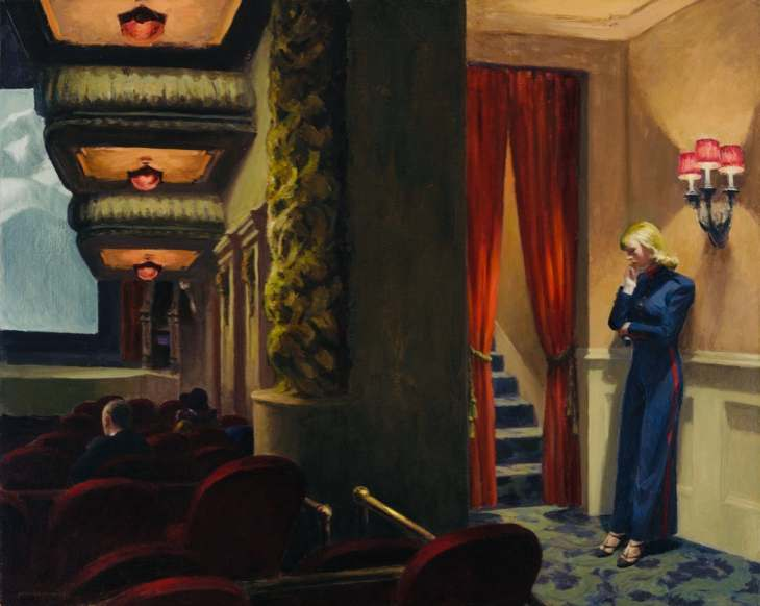
\includegraphics[width=2.96404in,height=2.36319in]{figuras/hopper-new-york-moview-1939.pdf.compressed.pdf}
  \figurenote{Fonte: \hiperlink{moma.org}{Museu Moma}}
  \end{minipage}
\end{figure}

No artigo sobre a noção de três espaços, \textcite{borges2019sobre}
comenta a relação com o espaço em Rohmer, que por ter uma função mais
didática, não contemplaria a complexidade da relação entre espaço e
tempo do cinema. No entanto, priorizamos nesta pesquisa a dimensão
espacial. Intuímos que nas teorias do cinema sobre a construção do
espaço cinematográfico encontraremos bases para a compreensão da
relação entre o artista e a imagem que constrói. Portanto, a partir de
agora avançamos nossa investigação para o pensamento de dois teóricos
do cinema, dos nossos tempos: Jacques Aumont e André Gardies. Na outra
ponta, percorremos textos de Delfim Sardo em uma teoria que aborda
questões mais amplas ligadas à arte em geral.

\subsection{O cineasta pintor --- a teoria crítica em Jacques Aumont}%
\label{o-cineasta-pintor-a-teoria-cruxedtica-em-jacques-aumont}

Estudioso do cinema, e das relações entre o cinema e a pintura, Jacques
Aumont, em seu ensaio sobre o pictórico e o fílmico, aponta alguns
caminhos interessantes para se pensar o que o cinema absorveu da
pintura, ao escrever sobre Lumière, considerado um dos criadores do
cinema. \citeauthor{aumont2004olho} faz~uma análise do homem que propagou a imagem filmada,
projetada e apresentada ao espectador em uma~sala de cinema. No
primeiro capítulo de \emph{O olho interminável}, o autor qualifica
Lumière como \emph{o último pintor impressionista}, fazendo referência
à fala de Godard neste sentido, em dois momentos: 1966 em uma
retrospectiva Lumière e em 1967, por meio de uma personagem do filme
\emph{A chinesa}. Ao fazer isso, Aumont descreve um dos encontros
fundamentais do cinema com a pintura, quando ambos trazem naquele
momento a ideia de buscar a impressão de realidade \parencite[27]{aumont2004olho}.

A problemática relacionada ao espaço, ao movimento e à narrativa, se
subjuga aos limites do quadro e resolve caminhar para dentro do espaço
diegético ou das imagens em perspectiva criadas por estratégias da
pintura, como nos conta Aumont em \emph{O olho interminável} (2004).
Podemos afirmar que por meio destas estratégias, o autor do filme
encontra abertura relativamente suficiente para expandir e representar
o mundo sem limites das imagens de sua mente.

\textcite{aumont2004olho} nos conta que Bazin (1951), no texto \emph{Pintura e
	cinema}, constata que Resnais, em diversos filmes,
\enquote{\enquote{\emph{abriu}} o espaço das telas pintadas, dotou-o de
	um fora imaginável, de um fora-de-campo.} E passa a refletir sobre
aspectos do quadro partindo do seguinte:

\begin{displaycquote}[142]{aumont2004olho}[.]
	O quadro fílmico, por si só, é centrífugo: ele leva o olhar para longe
	do centro, para além de suas bordas; ele pede, inelutavelmente, o
	fora-de-campo, a ficcionalização do não-visto. Ao contrário, o quadro
	pictórico é \emph{centrípeto}: ele fecha a tela pintada sobre o espaço
	de sua própria matéria e de sua própria composição; obriga o olhar do
	espectador a voltar sem parar para o interior, a ver menos uma cena
	ficcional do que uma pintura, uma tela pintada, \emph{pintura}
\end{displaycquote}

O espaço das imagens pictóricas e fílmicas de que trata Aumont é o
espaço que é visto e não o espaço percebido, como são o movimento ou a
luz. Ele é construído a partir de percepções visuais,
cinésicas\footnote{Cinésica --- adjetivo relativo a cinesia-substantivo
	feminino --- capacidade de se movimentar = mobilidade, movimento.} e
táteis.

\begin{displaycquote}[113]{aumont2004olho}[.]
	Ver o espaço seria interpretar através de informações visuais
	relacionadas à profundidade ou terceira dimensão da imagem: altura,
	largura e profundidade. O quadro que visa ao \emph{trompe-l'oeil}, teve
	inúmeros elementos descritos já nas \enquote{\emph{regras de Leonardo}}: os
	objetos próximos parecem maiores, sua textura aparente é mais grossa,
	seus contornos mais claros, suas cores mais saturadas, eles parecem ser
	mais baixos, estar menos próximos do horizonte. Grosso modo, isso
	significa que no real como no quadro, a perspectiva linear, com o
	eventual auxílio da perspectiva \enquote{atmosférica}, permite perceber a
	profundidade, que ela é até mesmo, em suas diferentes formas, o único
	fator que permite percebê-la de modo idêntico no real e no quadro
\end{displaycquote}

Para ele, \enquote{é em termos de quadro que cinema e pintura têm a
	semelhança mais clara, talvez por ser a mais superficial, como tenderia
	a provar os pastiches e as citações de um pelo outro, quase sempre nos
	termos, fetichizados por muitos cineastas e muitos críticos, da
	composição} \parencite[123]{aumont2004olho}. Ele critica em Bazin, por meio de
exemplos, o mau gosto de termos como \enquote{planos-telas pintadas} e
\enquote{beleza pictórica no cinema}, relacionados a princípios da
composição harmoniosa. O filme \emph{Van Gogh}, de Alain Resnais,
produzido em 1948, é tratado como um caso célebre de filmes sobre a
pintura.\footnote{\url{https://www.youtube.com/watch?v=SmILXxGaXMo\&t=11s\&ab_channel=anthologiablog}}
Destacamos aqui parte da análise feita por Aumont, na qual
\emph{alfineta} Bazin por utilizar estes termos (o academismo dos
\enquote{planos-telas pintadas} devia ser absolutamente insuportável
para o cantor do neorrealismo). Entretanto, trata de forma poética a
evidência do quadro, ou da janela, dentro do filme.

\begin{displaycquote}[124]{aumont2004olho}[.]
	Se os Van Gogh filmados por Resnais começam a contar uma história, a
	abrir para um fora-de-campo, é, com certeza, em virtude da forte
	propensão narrativa do cinema, mas também porque a história começa --- e
	com ela a abertura --- nas telas pintadas. Se olharmos bem, não é por
	acaso que, em todas as versões de \emph{O quarto de Vincent em Arles},
	ambas as bordas laterais coincidem com uma porta (e verdade que Resnais
	nos faz passar pela janela\ldots): uma evidenciação do quadro como abertura
	que encontramos, em formas cada uma mais visível do que a outra, em uma
	enorme proporção de telas pintadas do século XIX\@.\footnote{Recentemente
		restaurado, este curta de 1948 que ultrapassa limites, evoca
		brilhantemente a vida de Vincent Van Gogh, usando apenas suas pinturas
		como visuais \textcquote{icarus2022vangogh}[.]{\emph{VAN GOGH} traça a vida e a obra do grande
			pintor, desde seus primeiros dias como realista na Holanda, até sua
			estadia em Paris, o auge de sua carreira na Provença, e depois os dias
			sombrios de loucura que caíram sobre ele}}
\end{displaycquote}

\textcite[124]{aumont2004olho} argumenta que \enquote{os efeitos de quadro pensáveis são
	os mesmos em pintura e no cinema, mas o que difere são os meios
	empregados para atingir tais efeitos e, por conseguinte, os contextos
	estético-estilísticos nos quais são pensados.}  A partir desta
afirmação, se refere aqui à falta de tratamento por teóricos como
Arnheim e Eisenstein, de efeitos como os princípios de enquadramento do
estilo clássico hollywoodiano, que produziu uma quantidade esmagadora
de planos \enquote{centralizados}, ou seja, que utilizam muito pouco as
bordas do quadro. Somente com a análise \emph{neoformalista}, como a de
David Bordwell (1985), esta questão é aprofundada. A diversidade de
estilos relacionados a estética e teorias muito antigas como a do
\emph{centro de simetria}, trazidas da pintura, são tratadas como
fórmulas,~tal qual a das personagens refletidas no espelho de ambos os
lados do eixo vertical. Estas fórmulas
\textcquote[125-126]{aumont2004olho}[.]{encontram os lugares-comuns
	simbólicos ligados ao binário, ao duplo, ao ternário, e é com razão que
	os primeiros teóricos da abstração pictórica tiveram a sensação de
	estar apenas evidenciando leis muito antigas, até então implícitas}.%

Discussões sobre centralização e enquadramento, descentralização (o
centro esvaziado de qualquer personagem) e desenquadramento, envolvendo
cineastas como Antonioni ou Straub, apontam para uma diferença entre o
cinema e a pintura. Segundo \textcite{aumont2004olho}, esta diferença
se relaciona à impossibilidade da cultura visual ocidental de
\textcquote[129]{aumont2004olho}{separar a janela e o limite, a
	profundidade fictícia e a superfície real \textelp{} uma dupla e
	indissociável natureza da imagens}. Ele nos conta que para Arnheim as
diversas modalidades da descentralização não passariam de um
\enquote{avesso da centralização}, ao que Pascal Bonitzer, em seus
artigos sobre filmes que usam a descentralização, irá contrapor com a
definição do desenquadramento \parencite[2019]{aumont2004olho}. Desenquadramento não é exatamente
descentralização \textelp{} primeiro, o desenquadramento suscita um
vazio no centro da imagem; segundo, ele remarca o quadro como borda da
imagem; terceiro, enfim, ele só pode se resolver na sequencialidade, e,
no cinema tende efetivamente a ela.
\parencite[Bonitzer \emph{in}][129]{aumont2004olho}

\citeauthor{aumont2004olho} acredita que o desenquadramento realiza o paradoxo de separar o filme de seu
fora-de-campo, o que é muito difícil de se fazer em pintura. Como
exemplo, cita as personagens cortadas pelo quadro, das telas de Degas.
\textcquote[134]{aumont2004olho}{Quando Degas corta, na borda do quadro, o rosto de uma
	personagem, não temos dificuldade em completar imaginariamente.}.

\subsection{O espaço no cinema por André Gardies}%
\label{sec-espaco-cinema-gardies}

A elaboração do roteiro ou da narrativa, definido a partir de um único
aspecto ao qual chamamos de argumento principal, se apoia primeiramente
na estruturação do espaço, como defende \textcite{gardies2019espaco}, a
despeito das imensas possibilidades temporais relacionadas à montagem.
Se quisermos construir uma pintura partindo de uma estrutura peculiar
do cinema não podemos deixar de nos aprofundar neste conceito.

Segundo \textcite{gardies2019espaco} o espaço é estudado no cinema a
partir de duas concepções dominantes: geográfica e plástica. Nos
interessa esta aproximação com um outro campo de pesquisa, onde
teóricos da geografia realizam análises vinculadas a espaços fílmicos
sobre a cidade, a natureza ou a geografia do western, que se articulam
pelo lado do cinema com a estética de uma época, de um gênero ou autor.

Como vimos em Rohmer, a concepção plástica da cena é articulada
prioritariamente com estratégias ligadas à composição da imagem, muitas
vezes importada da pintura. A ideia da geografia nos leva a pensar
sobre o conceito de \emph{lugar} e em última instância, sobre o
deslocamento entre espaços (como veremos adiante, presente
metaforicamente em minhas pinturas da mala). Segundo
\textcite{martins2014estrategias}, ao refletir sobre espaço, território
e dispositivo:

\begin{displaycquote}[9]{martins2014estrategias}[.]
	Uma forma muito comum de pensar a questão espacial no cinema é a partir
	do conceito de lugar (quase sempre associado às locações). Para Gardies,
	lugar se define como o local que aparece com uma forma significante,
	delimitada por sua estrutura espacial --- tamanho, orientação, dimensões
	--- e por sua ordenação estilística --- objetos que o compõem, traços de
	estilo
\end{displaycquote}

Já o termo \emph{espaço}, refere-se à sala de cinema, ao ecrã, o que
ocorre no ecrã e, muitas vezes, vai além dele (espaço fora do ecrã). O
conceito de dispositivo, é usado por Gardies para agrupar estes
elementos, visando sistematizar os estudos sobre o espaço
cinematográfico. Dispositivo cinematográfico é um termo cunhado por
Baudry (1978) relacionado ao ato espectatorial, incluindo os espaços da
sala de cinema, da cabine de projeção e o ecrã \parencite{martins2014estrategias}.

A estrutura criada por \textcite{gardies2019espaco}\footnote{Textos do
	livro de \textcite{gardies2019espaco} traduzidos por nós.} caracteriza
o Espaço Cinematográfico por meio da noção de dispositivos presentes na
sala do cinema (cenográfico e especular). O \emph{Hall} é um espaço que
faz uma transição suave entre o espaço urbano e o espaço da sala de
cinema. A mudança do espaço da rua é suave porque o \emph{Hall} traz
características dos dois espaços: é fechado, mas permite a livre
circulação; ainda apresenta elementos visuais e os ruídos
característicos da rua, mas ele já cria um percurso que direciona para
a sala de cinema. Para Gardies, quando o espectador atravessa o
\emph{Hall} e chega à sala de cinema: o sujeito inscrito na ordem
cotidiana cede seu lugar ao sujeito \emph{espetacular,} devido às
restrições físicas da sala do espetáculo \parencite[18-20]{gardies2019espaco}.

O espaço do \emph{ecrã} interage com o olho espectador elaborando
concretamente uma organização topográfica, com conotações a partir dos
saberes espectatoriais relativos aos lugares representados. A
\emph{tela} é um espaço real à dupla visão: ela possui uma
materialidade física que o espectador percebe no início da projeção.
Quando tudo fica escuro e as primeiras imagens aparecem há outra
realidade, mais complexa e muito mais difícil de estabelecer, que surge
no \emph{ecrã}. Durante um tempo realmente perceptível, no qual o olho
do espectador se precipita para o centro da tela durante a projeção,
uma mutação radical se impõe em consequência do \emph{status} de
realidade da tela: sua materialidade física se transforma em uma
realidade imaginária cuja ilusão funciona de modo proporcional ao
prazer experimentado pelo espectador \parencite[22]{gardies2019espaco}.

Outros dois conceitos trazidos por \textcite{gardies2019espaco} são
\enquote{os processos de construção do espaço diegético e o papel
	narrativo deste.} A diegese se define como tudo o que pertence á
história contada, ao mundo proposto pela ficção do filme. Para ele o
espectador acessa o mundo diegético por meio de pré-requisitos, como os
dispositivos cenográficos construídos pela produção fílmica, que lhe
são oferecidos na bilheteria do cinema. Mas não apenas isto: o que o
espectador adquire na compra do ticket é um contrato fictício, com o
qual construirá, a partir de sua experiência e das proposições
fílmicas, um novo mundo. \enquote{Se cabe ao filme apresentar
	\emph{propostas}, cabe ao espectador a habilidade e o trabalho de
	fazê-las \emph{dar frutos}} \parencite[62]{gardies2019espaco}. Desta forma, Gardies demonstra o caráter
\emph{duplo} da construção do espaço diegético, representado não só
pelo próprio filme, mas também pelo espectador. Este mundo imaginário é
construído \emph{duplamente}: pelo próprio filme e pelo espectador. Ao
observarmos uma notícia falada em um rádio presente em uma cena,
estamos diante de um contexto diegético.

O realismo do espaço representado situa o espectador no mesmo tempo do
mundo quotidiano. Segundo \textcite{gardies2019espaco}, há uma inversão
do papel do voyeur que assina esse contrato na bilheteria: ele deixa de
procurar o mundo para usufruir de um mundo que vai até ele.

\begin{displaycquote}[67]{gardies2019espaco}[.]
	A experiência vivida do espaço, associada tanto à mobilidade do olhar do
	espectador quanto ao poder ordenador do olhar, me permite, a partir de
	dados fílmicos, construir (mas também \enquote{desconstruir}, rearranjar,
	transformar, reavaliar) constantemente, ao longo da projeção, o espaço
	diegético
\end{displaycquote}

No que tange a construção fílmica do espaço diegético,
\parencite[89]{gardies2019espaco} aborda a organismo do plano pelos
fotogramas e a realização do sintagma por meio da sucessão de planos.
Estas questões trataremos no próximo capítulo com a proposta de Block.
Entretanto, há que se destacar a importância atribuída ao papel
narrativo do espaço diegético por \textcite{gardies2019espaco} ao
trazer frames de filmes como \enquote{A Rosa Púrpura do Cairo}, de
Woody Allen (1985).

\subsection{Reflexões sobre espaço e óptica em Delfim Sardo}%
\label{reflexoes-espaco-delfim-sardo}

O teórico de arte contemporânea \textcite{sardo2017exercicio} trata da
questão óptica em seu livro O Exercício Experimental da Liberdade, no
capítulo \enquote{O enorme campo do que não tem nome}. Partindo da
premissa de que o \enquote{espaço tem sempre uma conotação metafórica,
	dependendo da forma como é descrito, vivido, pensado e
	conceptualizado}, \textcite{sardo2017exercicio} conceitualiza o espaço
passando por diversas abordagens. Para ele o espaço define a forma da
representação que produzimos no mundo. Mas centra no campo artístico a
verificação de suas ideias quanto à produção representacional do
espaço. Invoca as heterotopias de Foucault que fazem referência ao
teatro, como lugares onde coexistem espaços díspares. Desta forma
define o campo que lhe interessa, no caso o museu, como um espaço
heterotópico. Não nos interessa aqui avançar na questão do museu, mas
acreditamos que o lugar da teoria de Sardo, embora ligado a questões
tridimensionais, nos interessa para relacionar o espaço do cinema ao da
pintura \parencite[189-189]{sardo2017exercicio}.

Ao tratar da Vertigem, perturbação espacial relacionada à possibilidade
de queda, de instabilidade e de desequilíbrio, explica o entendimento
óptico-visual do espaço, e seu conceito descrito por Alois Riegl, na
história da arte, que entende a percepção do espaço arquitetônico como
sendo eminentemente óptico-visual. Esta visão se contrapõe ao
entendimento de que o espaço é a possibilidade de ocupação por um
corpo, para ser nele vivido. No século XX, o moderno na arquitetura
privilegia o entendimento do espaço óptico-visual em contraposição a
este espaço háptico-corporal, cuja história remonta à tese de 1914 de
Paul Frankl: \enquote{\emph{Principles of Arquitectural History, the
		four phases of architectural style.}}

Poderíamos pensar aqui tanto sobre as questões de \emph{estilo} na arte
trazidas por Wölfflin quanto as que Argan levanta ao tratar da arte
moderna sob o prisma da arquitetura. Afinal, o campo da arquitetura é o
mais ligado à ideia de construção. No entanto,
\textcite{sardo2017exercicio} introduz a ideia de \emph{ambiente},
ligada à expansão das artes de projeto:

\begin{displaycquote}[206]{sardo2017exercicio}[.]
	\textelp{} nomeadamente a arquitetura e o design nascente, para um modelo que
	produz outros mecanismos de representação do real entendido como espaço,
	isto é, como possibilidade. A obra de arte é uma ação sobre o real, que
	visa produzir um universo conectivo, participativo e vocativo
\end{displaycquote}

Cabe aqui uma reflexão: Como estaria sendo transformada a atmosfera
fílmica\footnote{No cinema a atmosfera pode ser fabricada através de
	meios fílmicos como direção de atores, o trabalho da luz, do som
	\textelp{} a utilização do for a-de-campo, a profundidade de campo
	\textelp{} No cinema a atmosfera é o que dá o \emph{tom} à
	representação. É ela que a caracteriza, atribuindo-lhe propriedades,
	qualidades e intensidades \parencite{gil2005atmosfera}. \emph{A atmosfera no cinema: o caso de
		\enquote{A sombra do caçador} de Charles Laugthon entre onirismo e
		realismo}. Fundaçāo Caluste Gulbenkian \& Fundação para a Ciência e
	Tecnologia.} na \enquote{caixa
	preta}\footcite[Segundo][40]{porras2010entre}[\enquote{designação usada
		para assinalar uma tipologia arquitetônica comumente utilizada na
		construção de espaços destinados a projeções de cinema, apresentações,
		concertos, etc.}] e nas imagens da pintura no \enquote{cubo
	branco}\footcite[Designação usada para indicar os espaços de exibição
	próprios das artes plásticas e/ou visuais, tais como museus e galerias.
	(p.~46)]{porras2010entre} depois do advento do celular? O espaço da
tela do cinema na sala escura e da pintura na galeria tem hoje uma
outra configuração, ao se tornar móvel e transitar por outros lugares.
Existe um novo espaço expositivo, de galerias, museus, feiras de arte e
sites de artistas, nascido no ciberespaço\footnote{Para Pierre Lévy
	(2010), \enquote{ciberespaço} é sinônimo de rede. \enquote{eu defino o
		ciberespaço como o espaço de comunicação aberto pela interconexão
		mundial dos computadores e das memórias dos computadores}. Do artigo
	\emph{Cibercultura Teatral: Panorama do trabalho criativo no
		ciberespaço em Porto Alegre durante a pandemia} DOI:
	10.14393/issn2358-3703.v8n2a2021-}, cuja imprevisibilidade de recepção
por parte do espectador se torna um novo desafio para o autor, tanto da
pintura tradicional quanto do cinema.

O capítulo \emph{Imagens, lentes, espaços e movimentos}, se inicia com
uma abordagem sobre o Atlas, de Gerhard Richter, tratando da fotografia
como substantivo coletivo, trazendo a experiência de Aby Warburg e seu
\emph{Atlas Mnemosyne}. Assim \textcite{sardo2017exercicio} explica as
\emph{constelações de sentido}, assentes na ideia de \emph{intervalo}
entre imagens, no espaço físico que as delimita e define. Importa aqui
o esclarecimento que \textcite{sardo2017exercicio} faz em relação ao
Movimento, ao apontar o que se segue, trazendo então o cinema para a
conversa:

\begin{displaycquote}[232]{sardo2017exercicio}[.]
	O problema do intervalo conhecia, entretanto, outros desenvolvimentos,
	nomeadamente com o surgimento do termo nos escritos de Sergei Eisenstein
	e Dziga Vertov. Esta questão, a que regressaremos no capítulo seguinte,
	merece aqui ser introduzida na forma como Vertov a define, ao centrar a
	arte do movimento não no movimento em si, mas \enquote{nos intervalos que levam
		o movimento a uma resolução cinética}
\end{displaycquote}

O contexto é o início de uma teoria cinematográfica sobre o intervalo,
durante o período de 1924--1930, nos textos soviéticos de Eisenstein e
Vertov, e no espaço europeu com Jean Epstein, Louis Delluc, Joris Ivens
e Hans Richter. A partir das imagens em constelações do Atlas de
Warburg (1926 --- conferência sobre Rembrandt) \footnote{Sobre Warburg
	e o cinema \url{https://labcom.ubi.pt/livro/314}}, a história de uma
teoria fotográfica que se relaciona ao cinema avança em questões
relacionadas ao espaço, ao intervalo, à profundidade e à imagem em
movimento, caminhando para a problemática da produção da serialidade,
que, segundo Sardo, é inaugurada pelos escritos de John Coplan (1968).
\enquote{O fotógrafo (à data, diretor da \enquote{\emph{Artforum}})
	define a \enquote{imagética serial} como um tipo de forma ou estrutura
	partilhada igualmente por cada trabalho num grupo de obras
	relacionadas, realizadas por um artista}
\parencite[233]{sardo2017exercicio}. O universo fotográfico teria recusado
a imagem única, no período surrealista de Man Ray, que usava séries que
deveriam ser vistas como conjuntos de estranheza instauradoras de
ambientes.


O termo \emph{laboratório}, que teria sido usado pela primeira vez na
apresentação de Aby Warburg (1927) ao estabelecer protocolos móveis e
experimentais na montagem de seu Atlas Mnemosyne, vem ao encontro das
questões processuais que levantamos em relação às possibilidades que o
pintor passa a elencar dentro do ateliê, uma espécie de
experimentalismo.

Acrescemos a este, um outro conceito, o da \emph{faktura}, com o qual
Sardo aborda a genealogia da imagem como compósito (colagem ou
fotomontagem), definido por David Burliuk no manifesto futurista de
1912, \emph{uma bofetada no gosto do público}. A palavra fatura é usada
como categoria estética efetiva, em referência à utilização de
materiais específicos a partir de um plano construtivo. O termo foi
usado para justificar não só questões ideológicas no período russo de
\emph{Rodchenko}, e também para a utilização de processos mecânicos de
produção, que não poderia ser objeto de assinatura (como ocorre na
pintura), \textcquote[238-239]{sardo2017exercicio}[.]{libertando a
	imagem de seu contexto de mercadoria para mergulhar no sistema de
	circulação social}. No entanto, queremos dar enfoque aqui ao uso da
palavra para traduzir o instrumental que o pintor lança māo para
instaurar suas próprias ideias, ainda que vinculadas a poéticas de
maior amplitude, seja com caráter social, político, mas
fundamentalmente baseado em sua própria compreensāo daquilo que está em
pauta no seu projeto. A fatura é, neste sentido, não só resultado das
reflexões do artista, mas também, de modo inverso, instrumento para a
criaçāo de sua poética.
